\section{The Implemention of the Translation}
\label{sec:owntool}
Our implementation of the translation is written as a plug-in to the ASAP tool. By making a plug-in to ASAP we can make use of the EMF CPN model and the CPN importer which makes it possible to import CPN models created in CPN Tools into the workspace. In the following we walk through the most important parts of the tool. Eclipse user would find the graphical user interface (see Fig.~\ref{fig:newproject}) familiar, since it looks very similar to the standard Eclipse IDE.

\begin{figure}[h!]
\centering
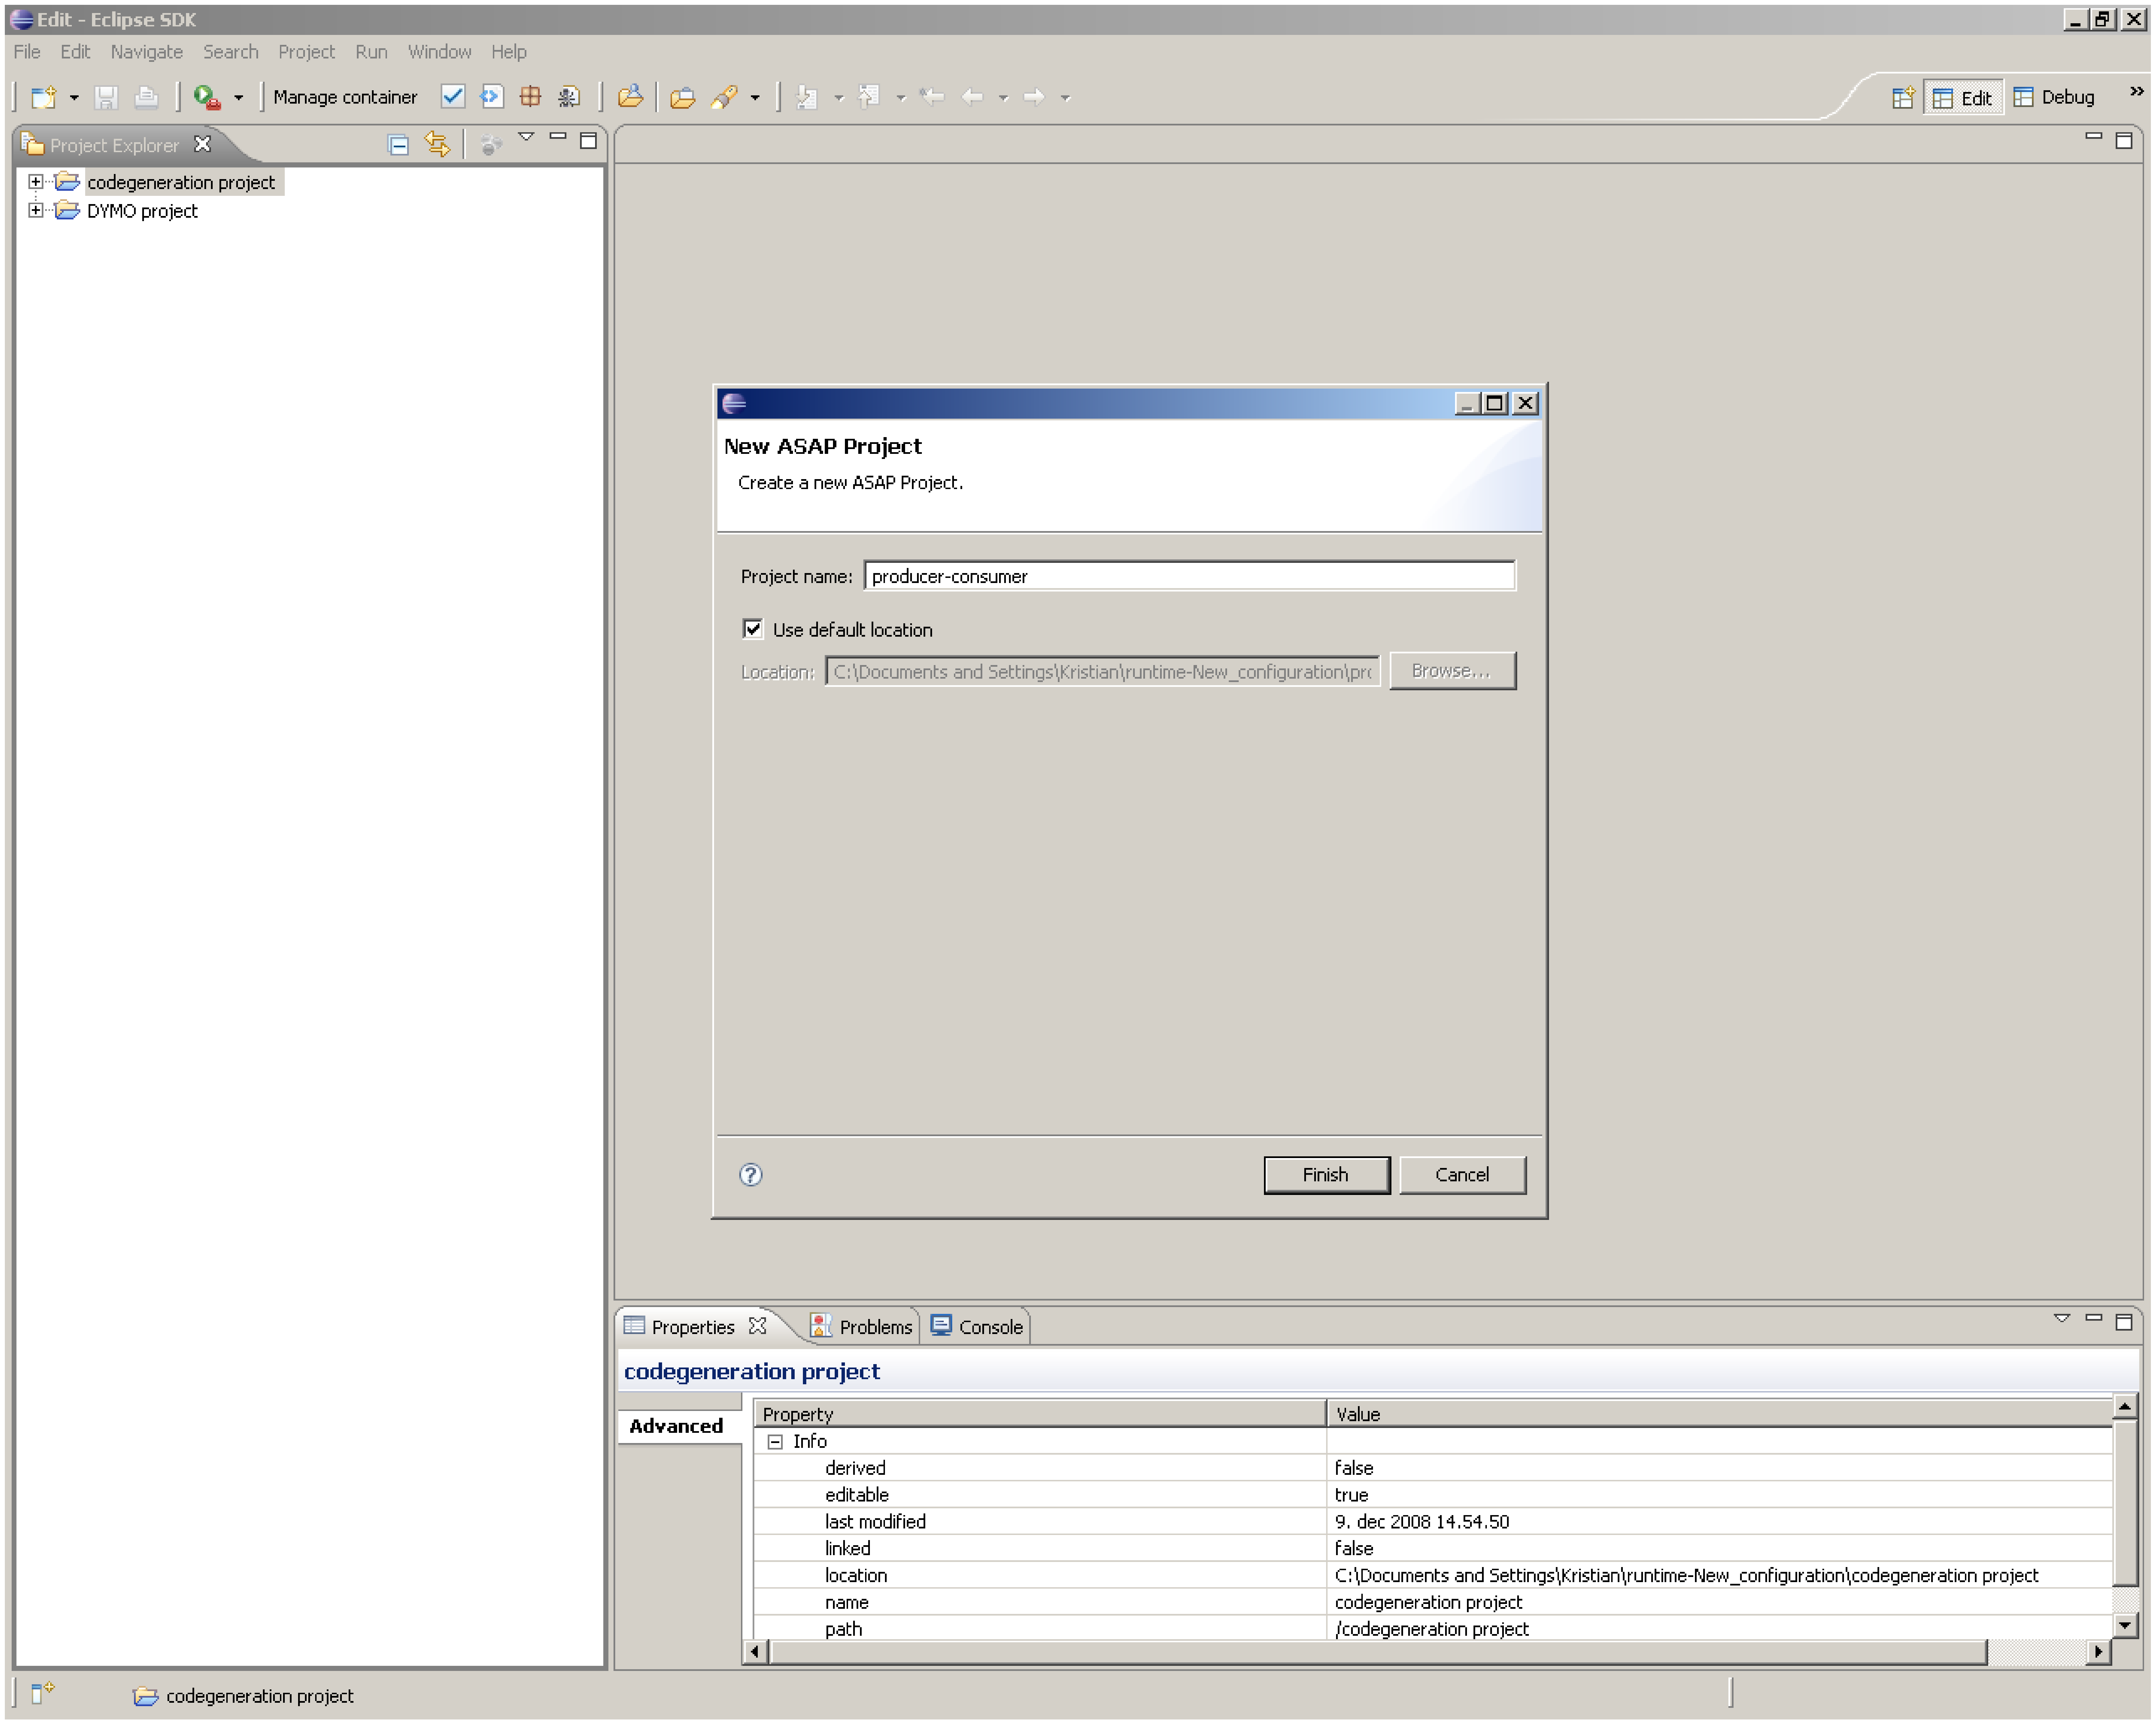
\includegraphics[width=\textwidth]{techniques_and_tool/graphics/newproject.eps}
\caption{The new ASAP project wizard}
\label{fig:newproject}
\end{figure}

To the left we see the \emph{project explorer}. To create a new project in the project explorer go to the \textbf{File} menu and choose \textbf{New} $\rightarrow$ \textbf{ASAP project}. The new ASAP project wizard will appear which is shown in Fig.~\ref{fig:newproject}. When the \textbf{Finish} button is pressed the wizard creates an ASAP project with the four folders \code{jobs}, \code{models}, \code{queries}, and \code{reports}. By right-clicking on the \textbf{models} folder it is possible to import models created in CPN Tools. The models are imported using the wizard shown in Fig.~\ref{fig:importcpn}. When the \textbf{Finish} button is pressed the CPN model is imported into the project and the folder \textbf{models} now contain the CPN model in a \code{.model} file which is an EMF model representation of the CPN model.

\begin{figure}[h!]
\centering
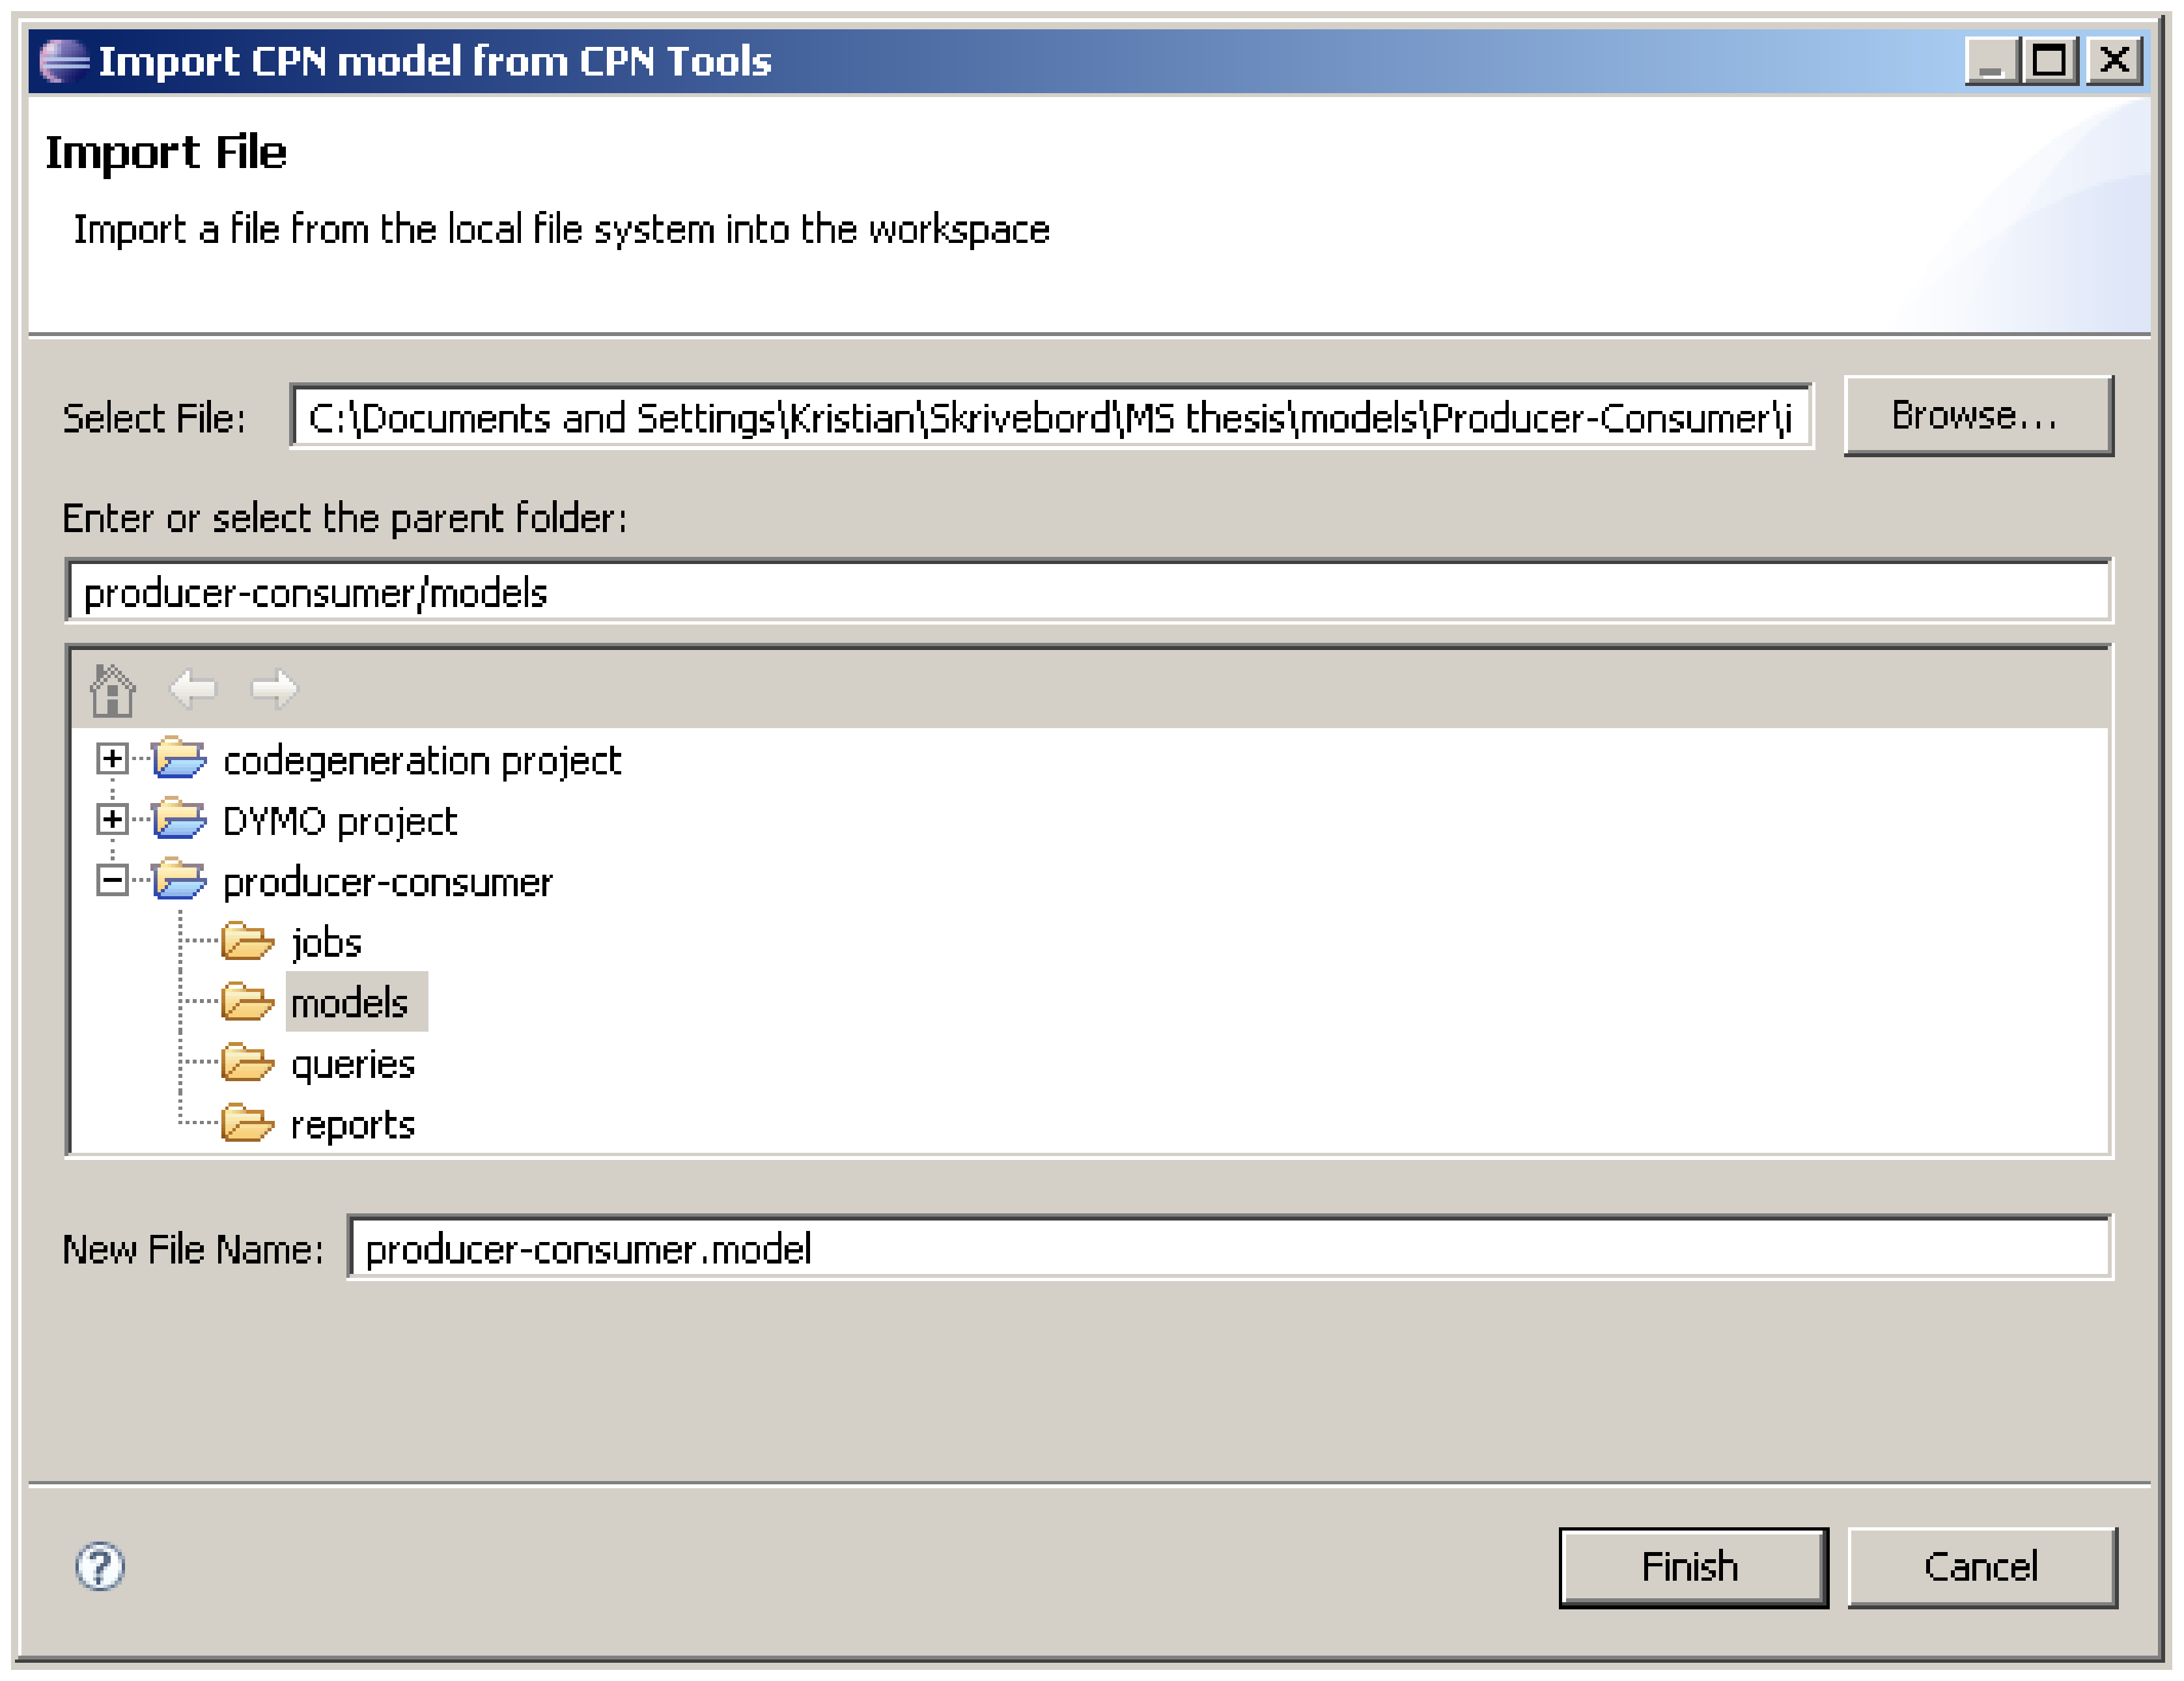
\includegraphics[scale=0.2]{techniques_and_tool/graphics/importcpn.eps}
\caption{The CPN model importer}
\label{fig:importcpn}
\end{figure}

We have added the possibility of right-clicking on a \code{.model} file, and choose \emph{Erlang code generation} which starts the wizard shown in Fig.~\ref{fig:cg1}. In this wizard the folder which will contain the generated code is given a name.

\begin{figure}[b!]
\centering
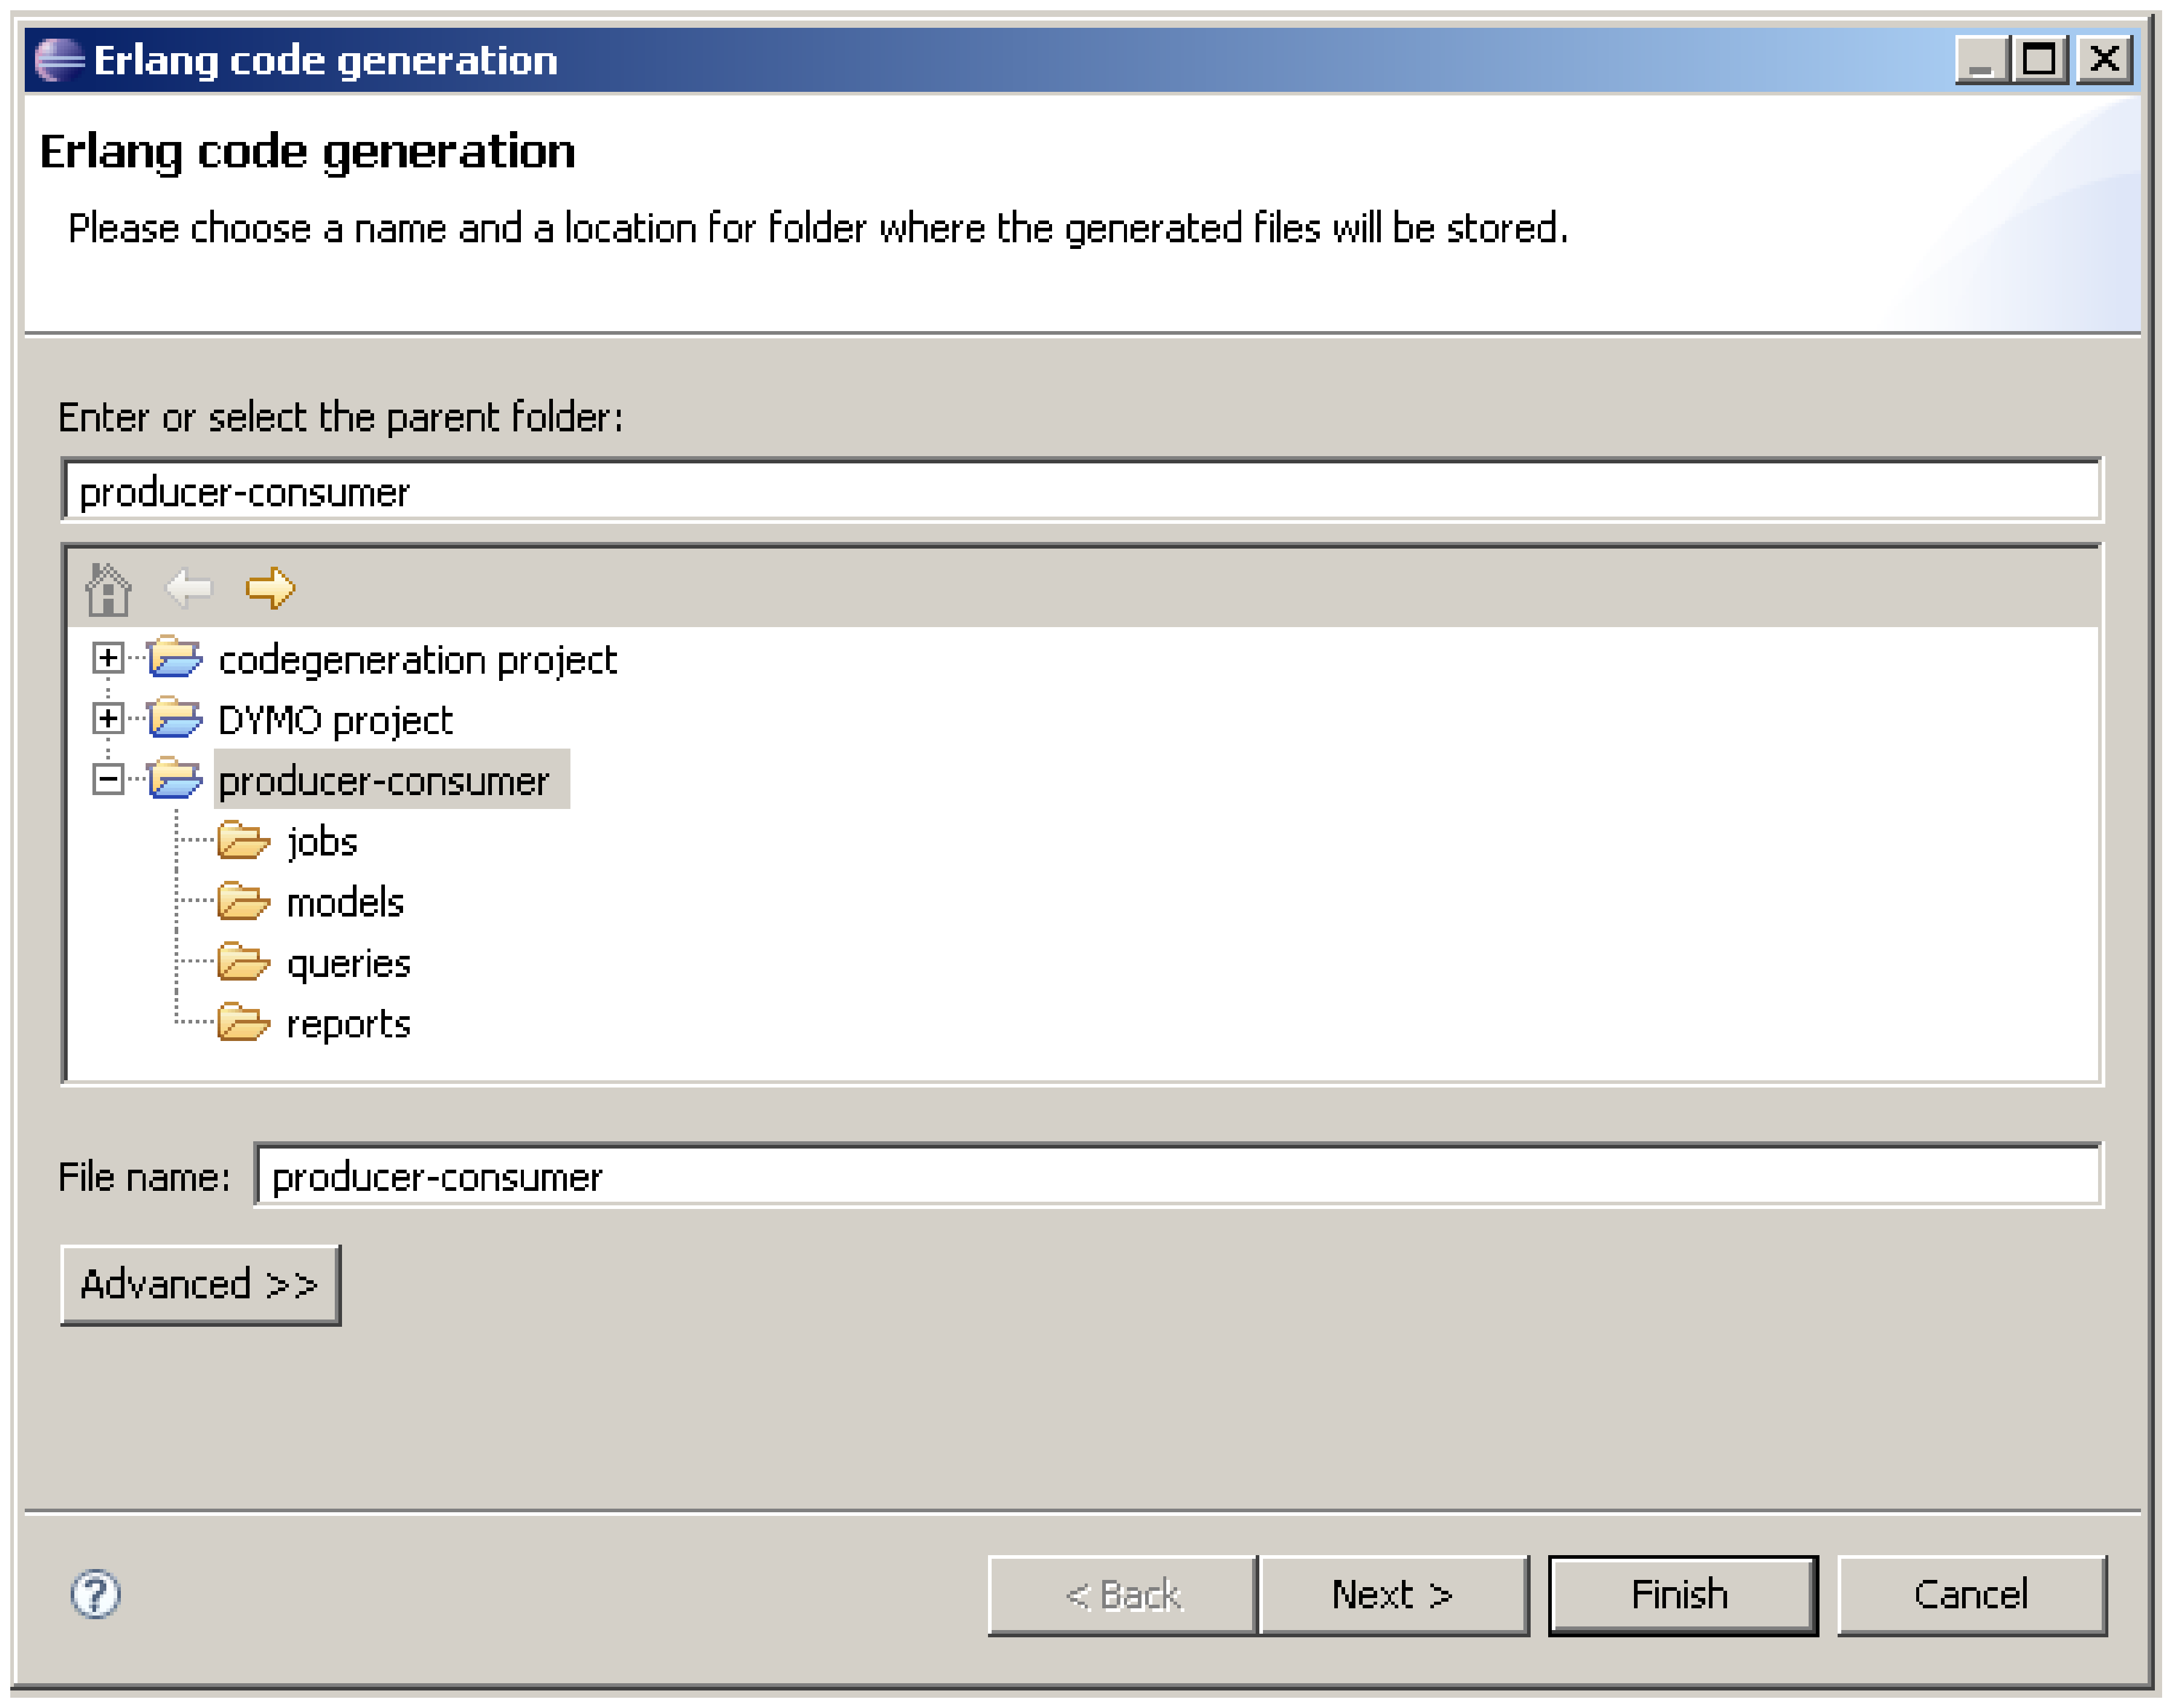
\includegraphics[scale=0.2]{techniques_and_tool/graphics/cg1.eps}
\caption{The code generator wizard step 1}
\label{fig:cg1}
\end{figure}

When pressing the \textbf{Next} button the screen in Fig.~\ref{fig:cg2} is shown. Here the user is able to choose which files should be generated by using the four check boxes in the top of the wizard. Below the CPN model to generate code from is chosen. When the \textbf{Finish} button is pressed the chosen files are generated and put into a folder as shown in Fig.~\ref{fig:cgprojectexplorer}.

\begin{figure}[h!]
\centering
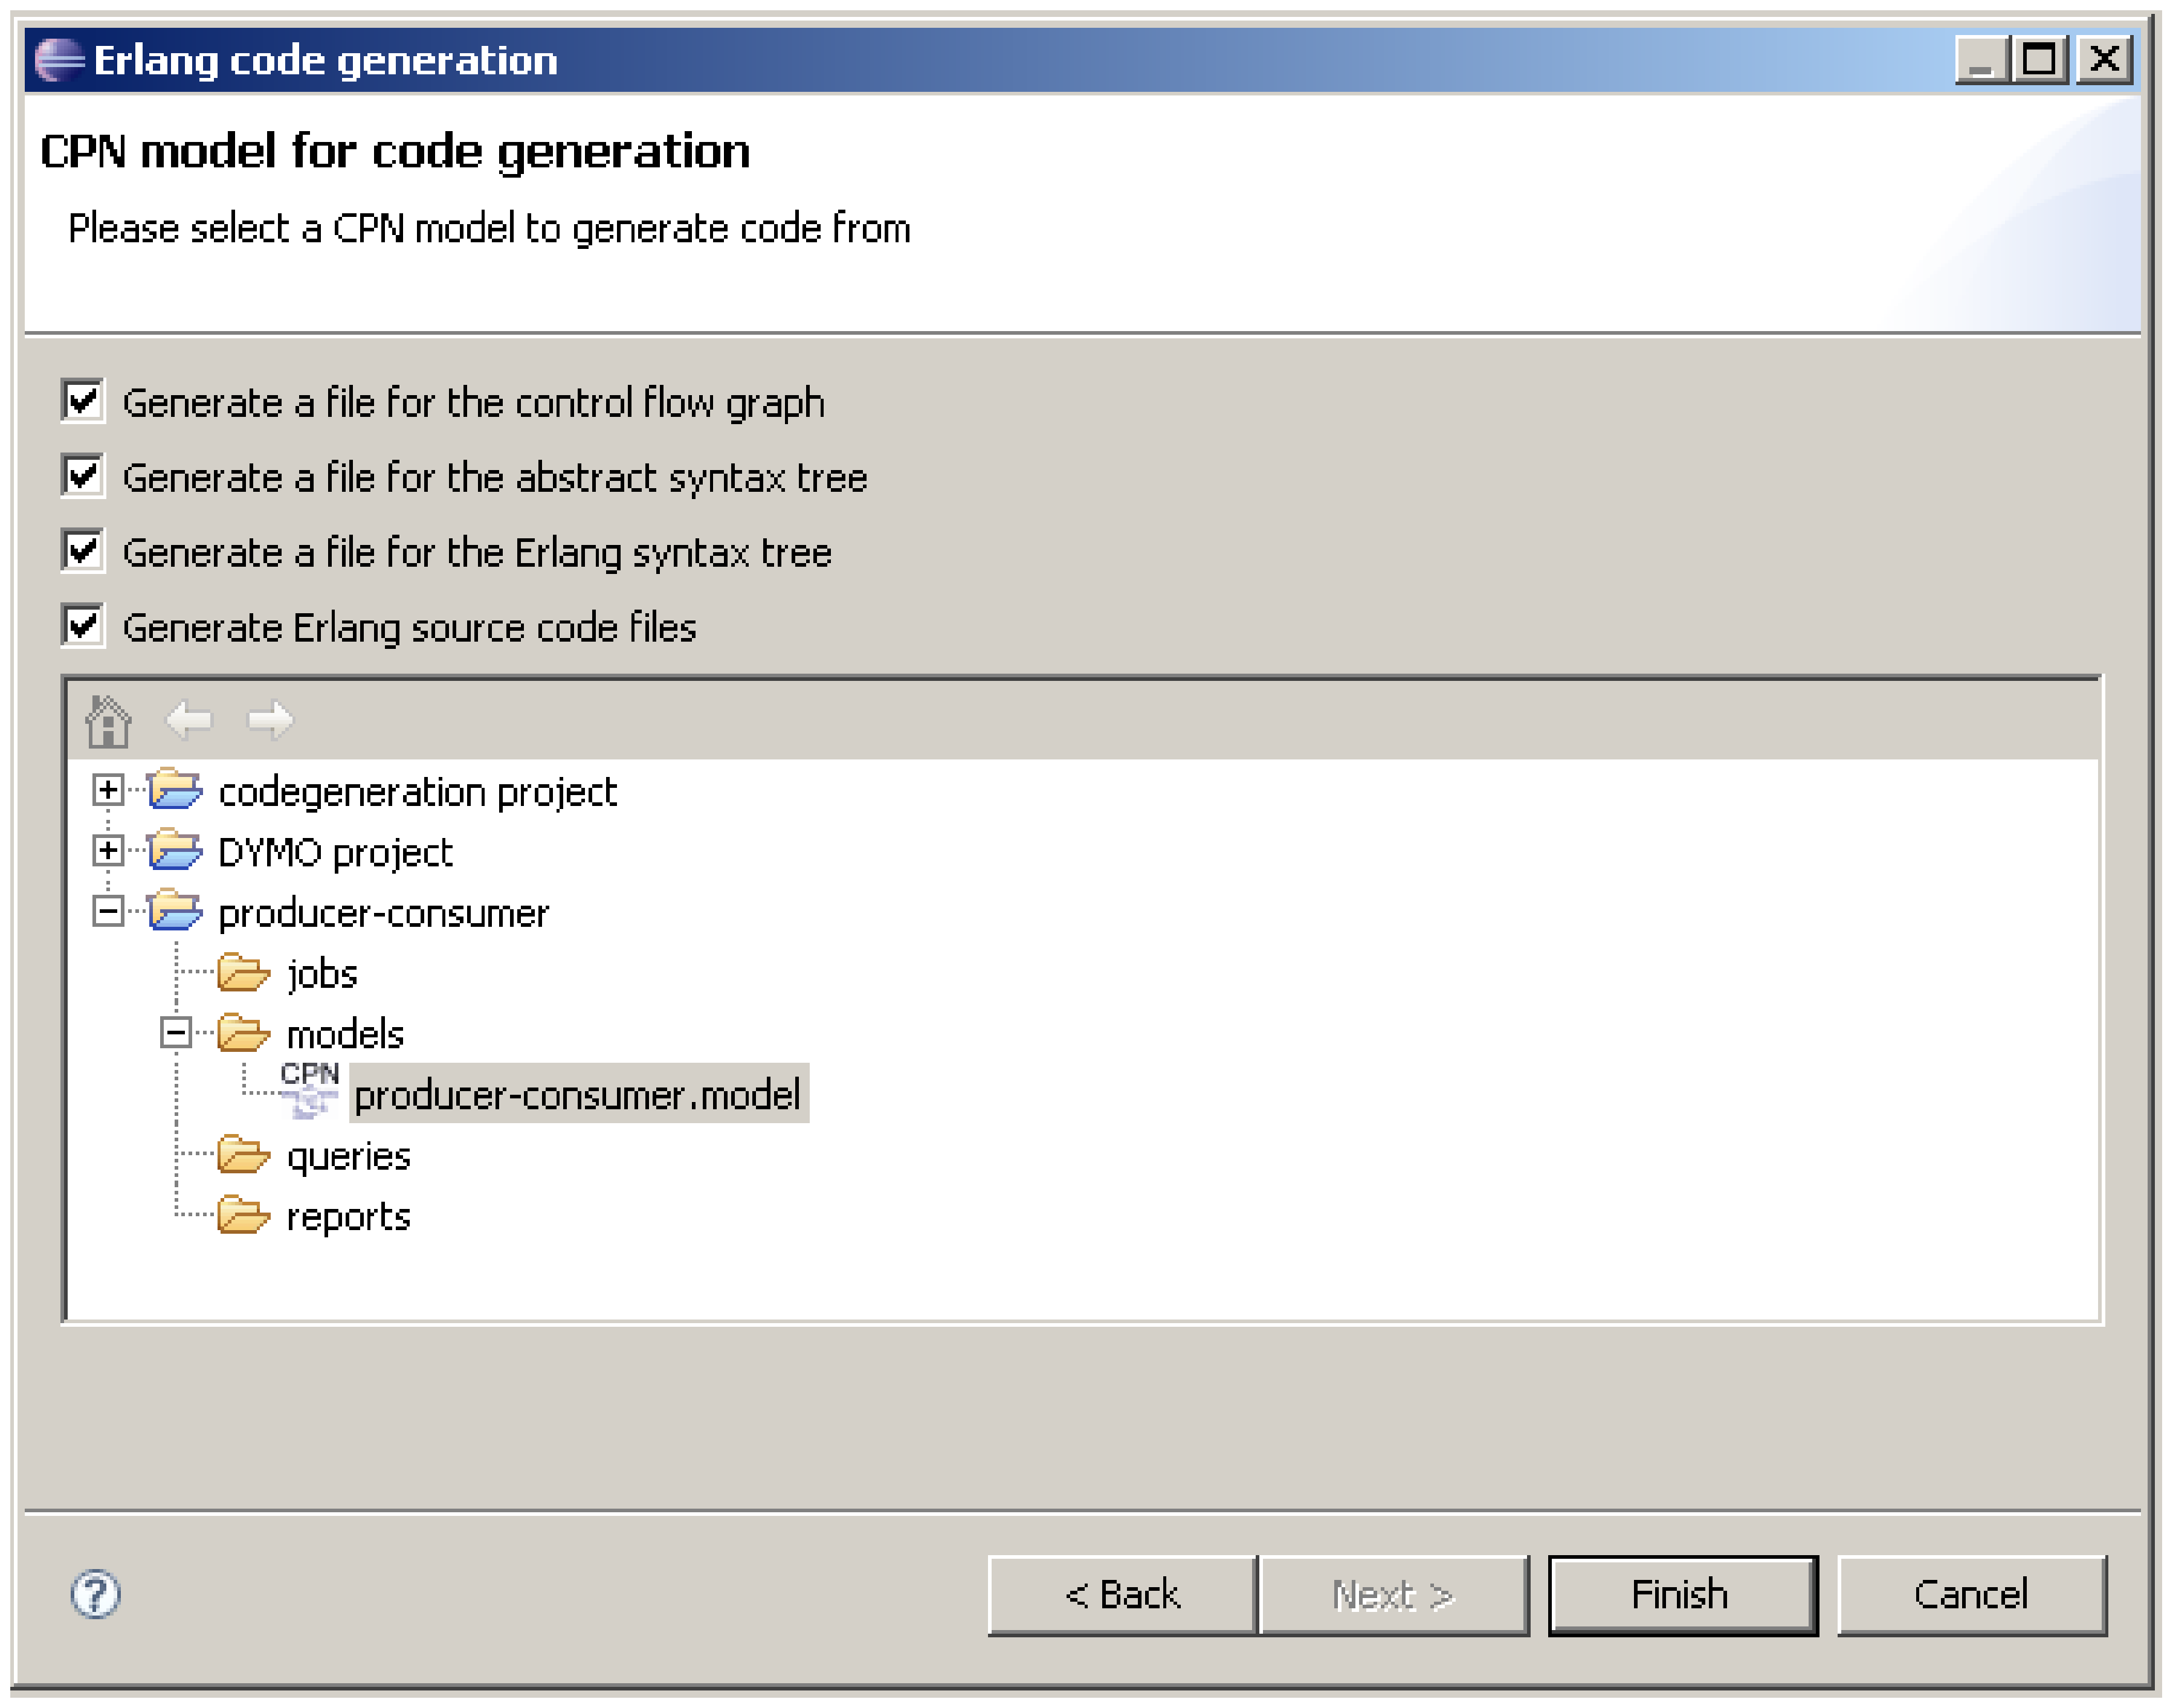
\includegraphics[scale=0.2]{techniques_and_tool/graphics/cg2.eps}
\caption{The code generator wizard step 2}
\label{fig:cg2}
\end{figure}

\begin{figure}[b!]
\centering
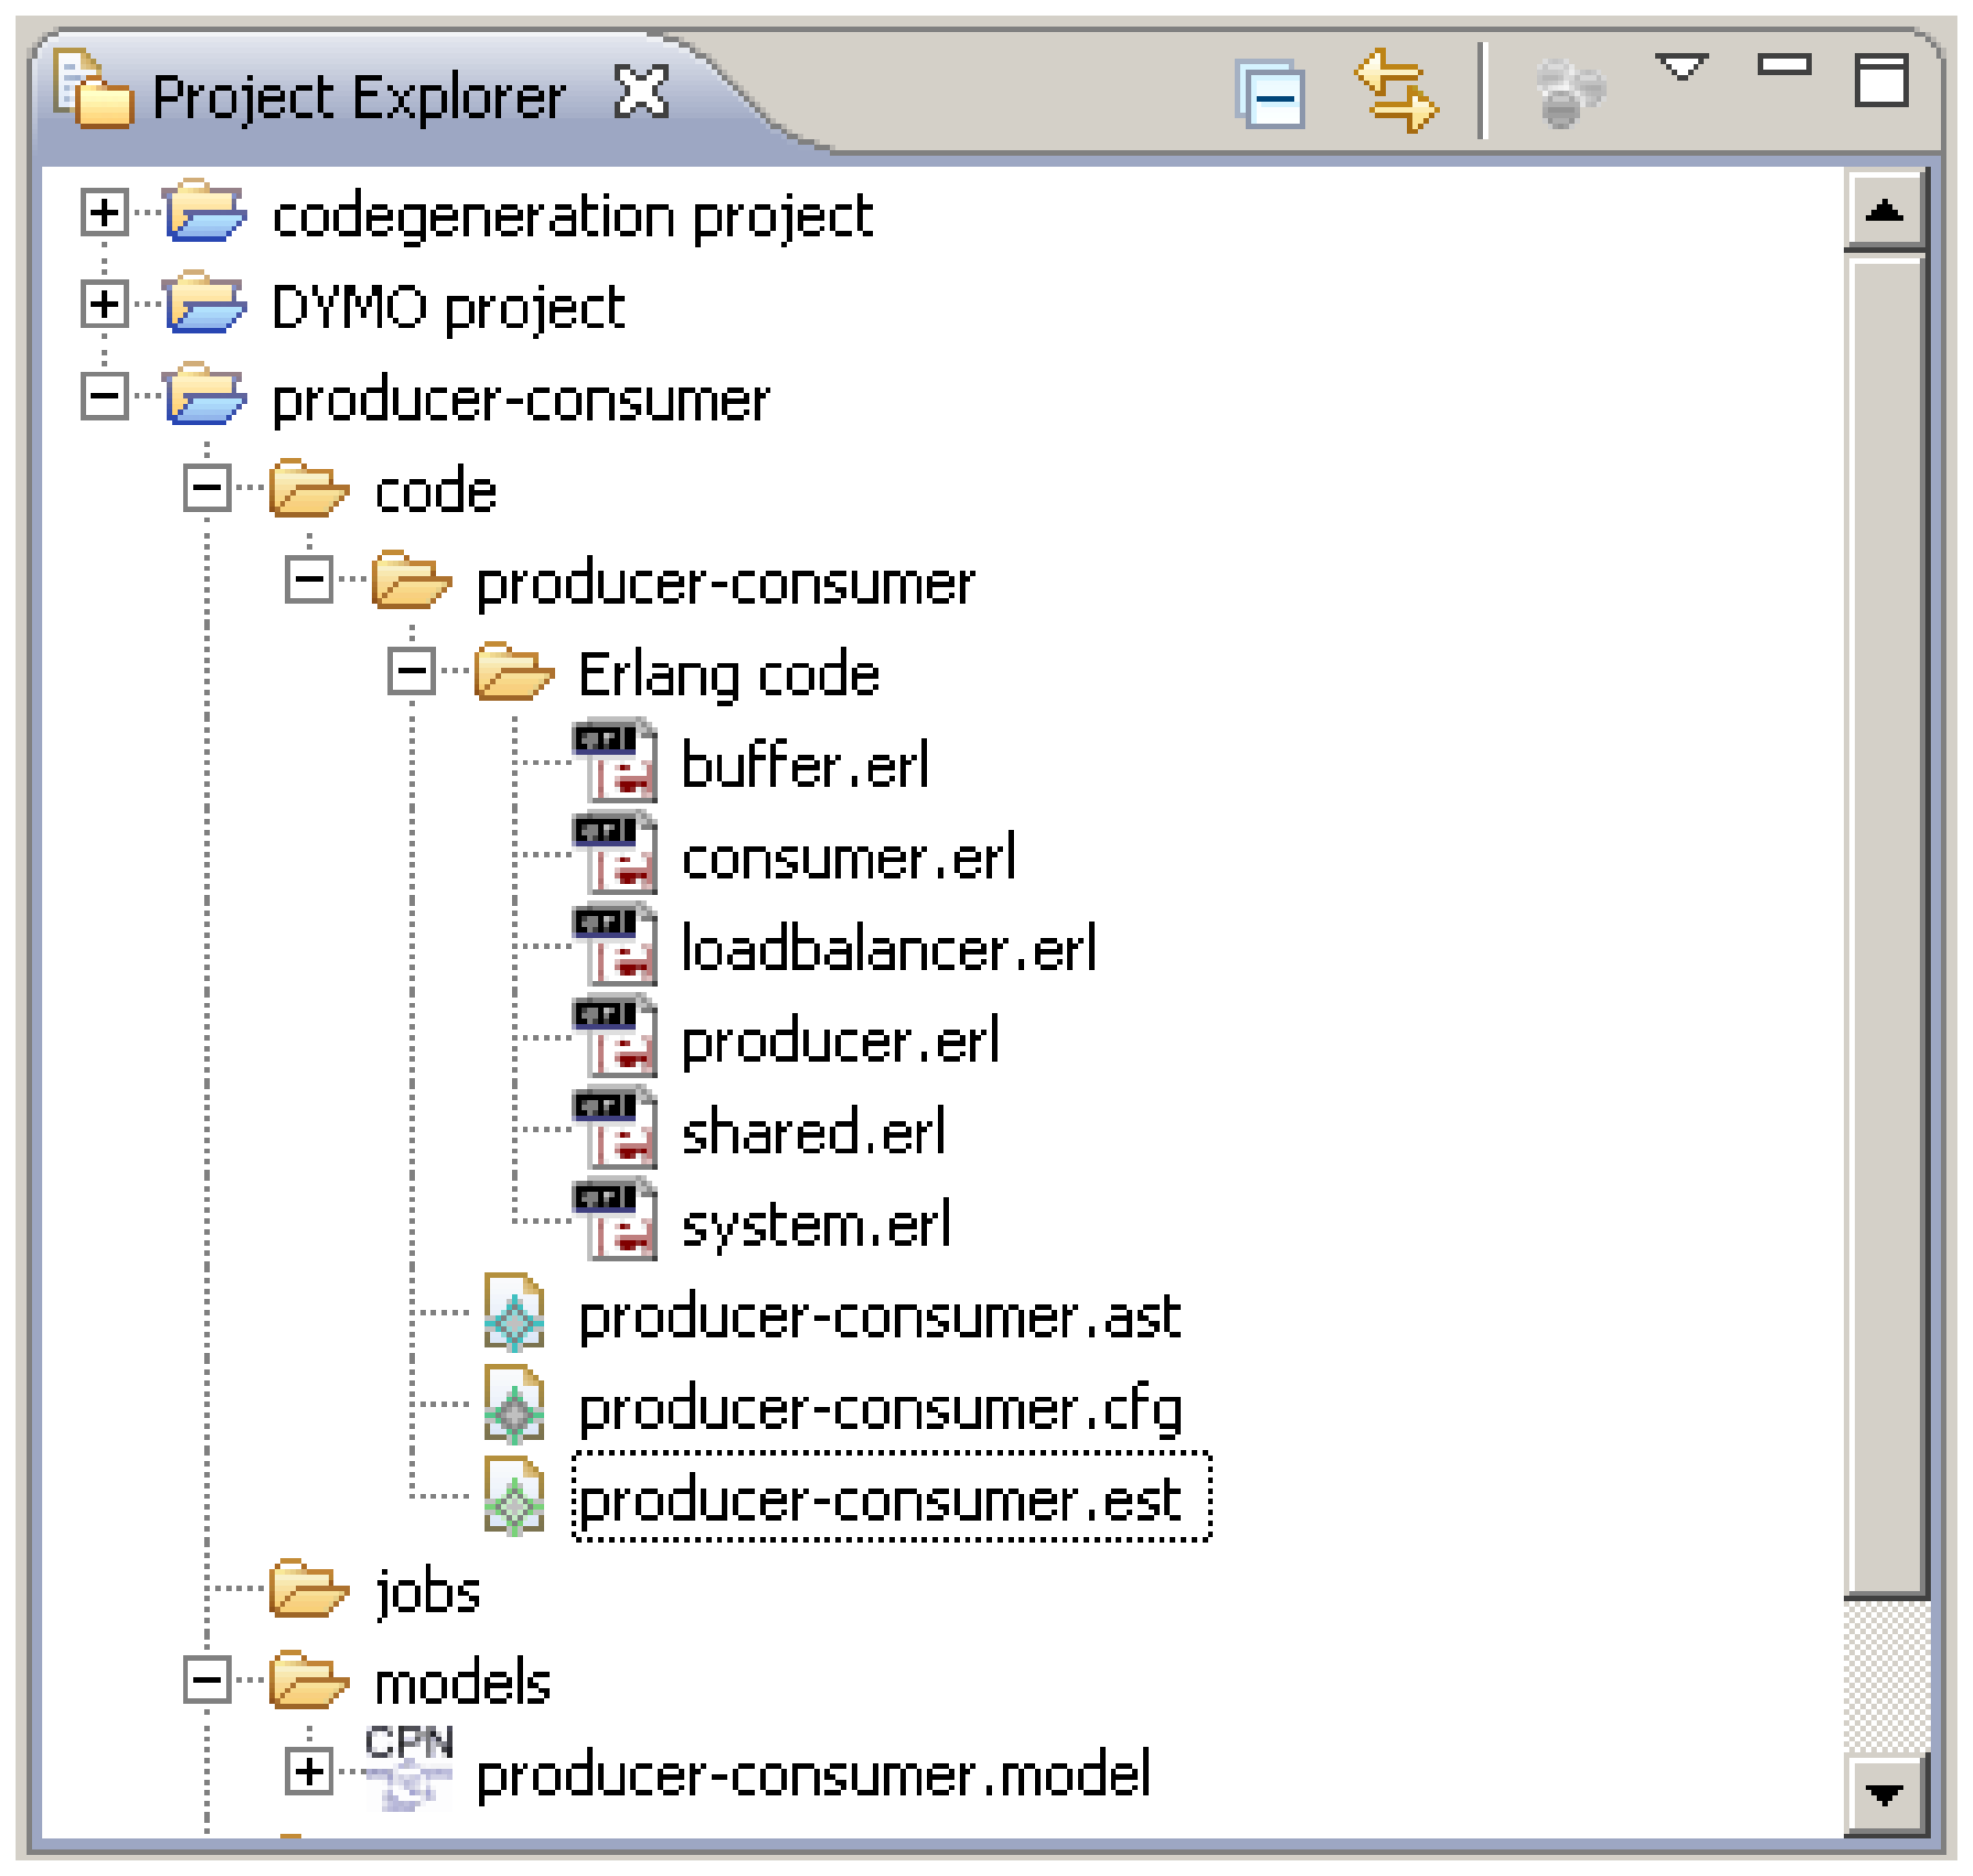
\includegraphics[scale=0.2]{techniques_and_tool/graphics/cgprojectexplorer.eps}
\caption{The project explorer after running the code generator wizard}
\label{fig:cgprojectexplorer}
\end{figure}

In the following we describe the generated abstract syntax tree (AST) from the producer-consumer system, which is represented as an EMF model. The control flow graph and the Erlang syntax tree are visualised in a similar way as the AST. The tree representation is shown in the tool, which can be used to inspect the different phases of the translation. In section \ref{sec:validateprodcons} we take a closer look at the generated code.

%\subsection{The EMF Control Flow Graph}
%In Fig.~\ref{fig:cgcfg} we find part of the generated CFG. We see that three process nodes are created; one for the producer, one for the consumer, and one for the load-balancer. We also see the global variable \code{Next Consumer}. We have unfolded the producer process, and we see that it contains three basic blocks: \code{Send Data}, \code{Produce Data} and \code{start}. Taking a closer look at the basic block \code{Produce Data} we see that it contains a read from, and a write to, the process variables \code{Data} and \code{PData}. The edge in the control flow graph from the basic block \code{Produce Data} and \code{Send Data} is represented in the basic block condition pair.
%
%\begin{figure}
%\centering
%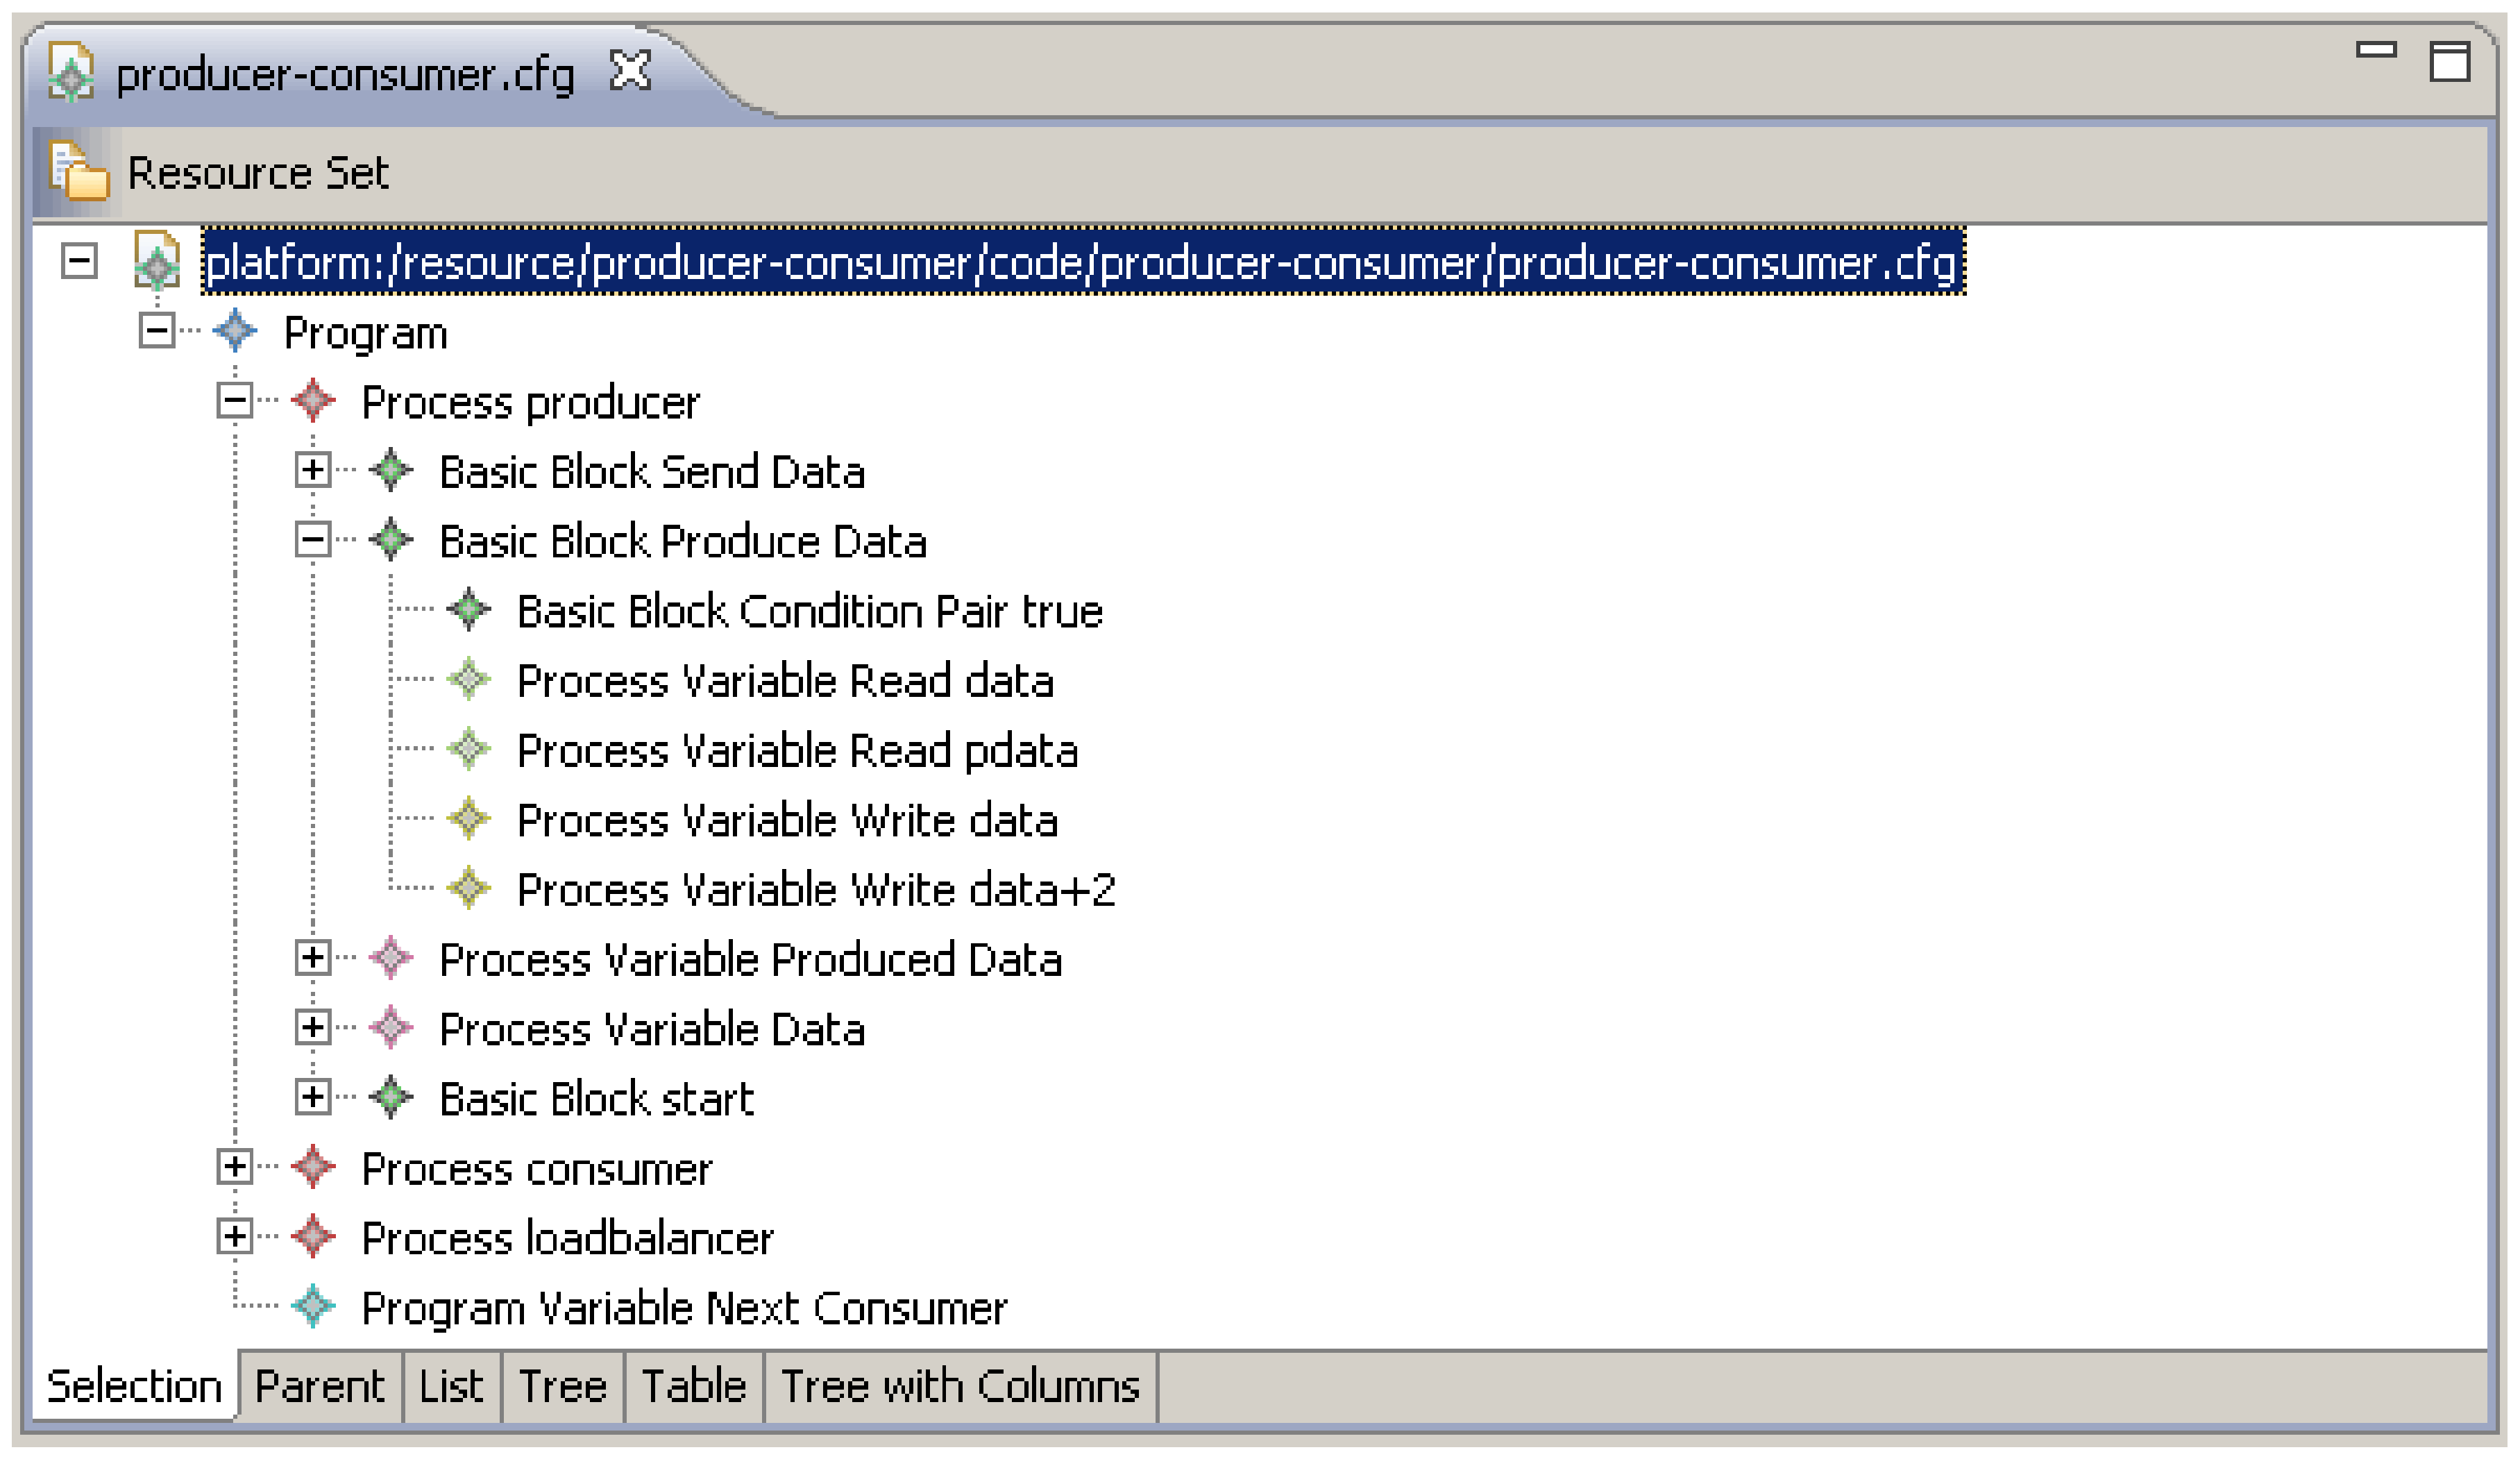
\includegraphics[scale=0.2]{techniques_and_tool/graphics/cfg.eps}
%\caption{The generated Control Flow Graph (CFG)}
%\label{fig:cgcfg}
%\end{figure}

\subsection{The EMF Abstract Syntax Tree}
In Fig.~\ref{fig:cgast} we show part of the generated AST. It contains the three processes: \code{producer}, \code{consumer} and \code{loadbalancer}. We see, that the initial expression of the global variable \code{Next Consumer} has been extracted. The initial expression is the integer constant \code{1} for \code{producer} instance one, and the integer constant \code{2} for producer instance two. Taking a closer look at the block \code{Produce Data} we see that two local variable declarations have been created. These are used in the read and write statements, e.g., we see the read statement where the value of the process variable \code{Data} is bound to the local variable declaration \code{data}. In the end of the block we see an unconditional goto statement.

\begin{figure}[b!]
\centering
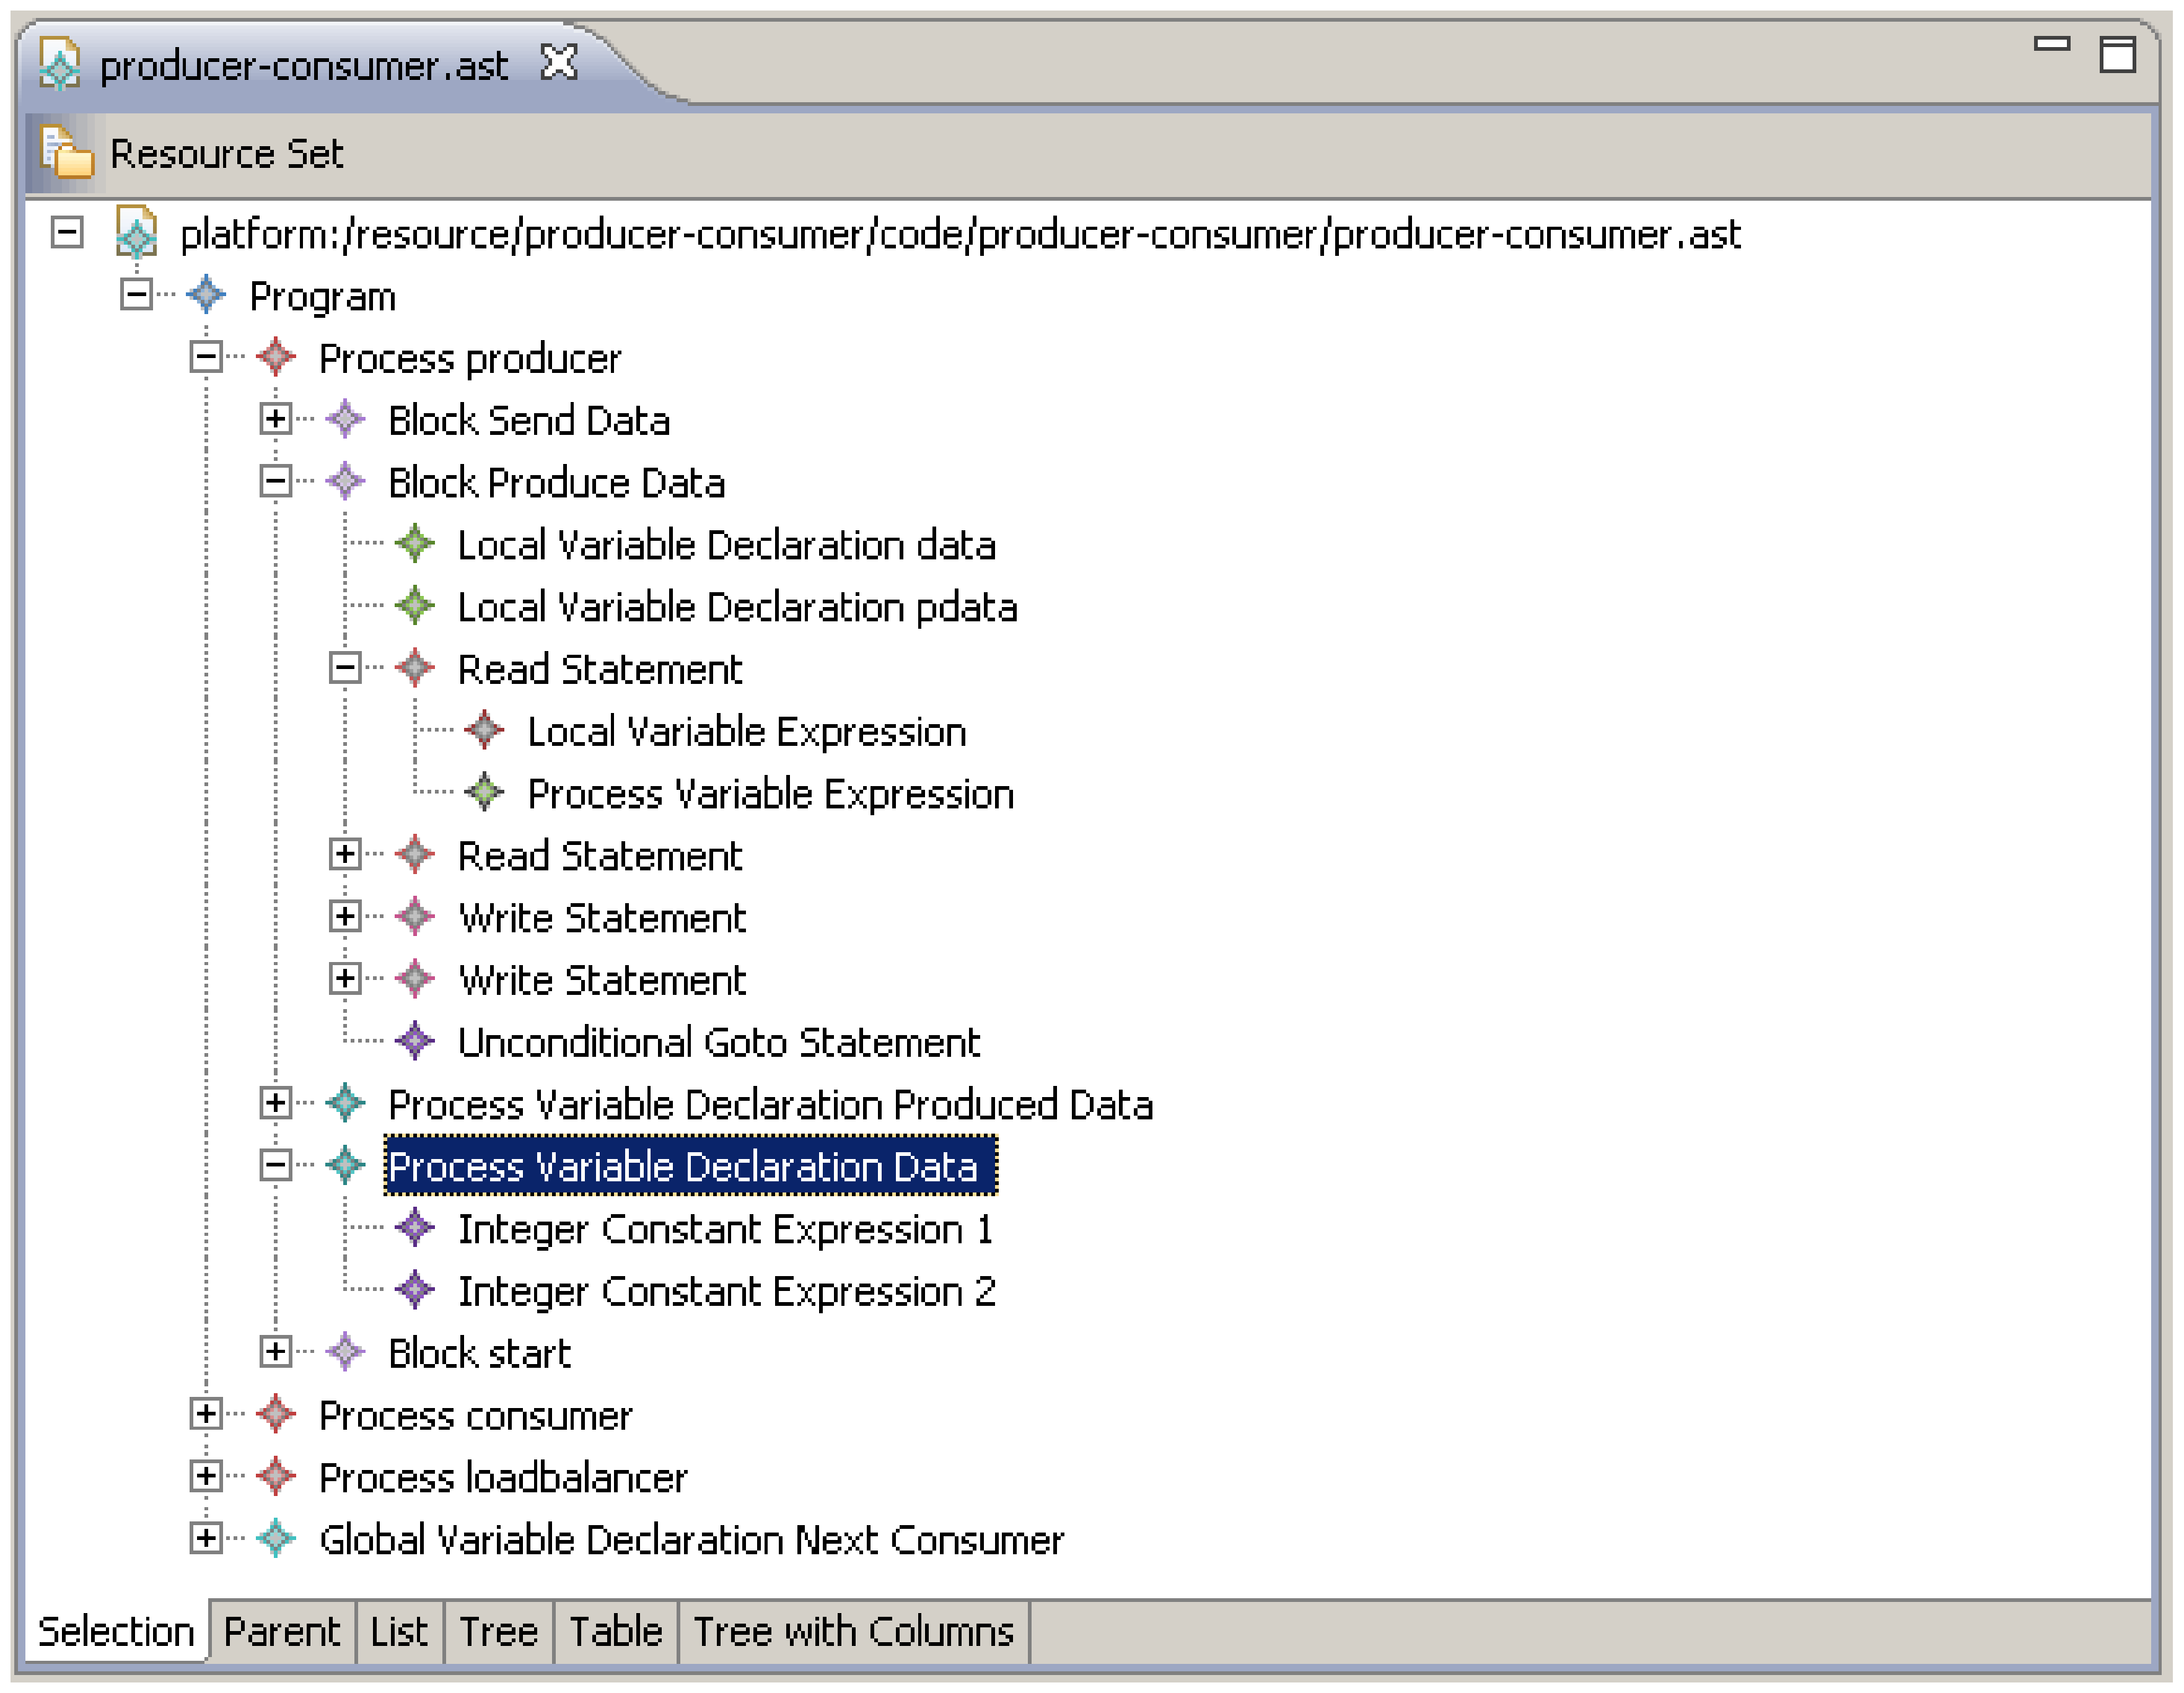
\includegraphics[scale=0.2]{techniques_and_tool/graphics/ast.eps}
\caption{The generated Abstract Syntax Tree (AST)}
\label{fig:cgast}
\end{figure}

%\subsection{The EMF Erlang Syntax Tree}
%In Fig.~\ref{fig:cgast} part of the EST is shown. In addition to the three module declarations for the producer, consumer and load-balancer, we see a system module and a shared module. The system module is responsible for spawning the process instances, and the shared module is used to share data as explained in \ref{TODO}. The module declaration for the producer is shown in some detail. We see the export attribute responsible for exporting the start function, and we also see the record declaration for the environment. It further more contains the three functions: \code{start}, \code{send\_data}, and \code{produce\_data}. Taking a closer look at the function declaration for \code{produce\_data}, we see the \code{Env} variable which is the argument to the function. We also see the match expression where the value of data is read from the environment. In the end of the function we see an application expression where the function \code{send\_data} is called.
%
%\begin{figure}
%\centering
%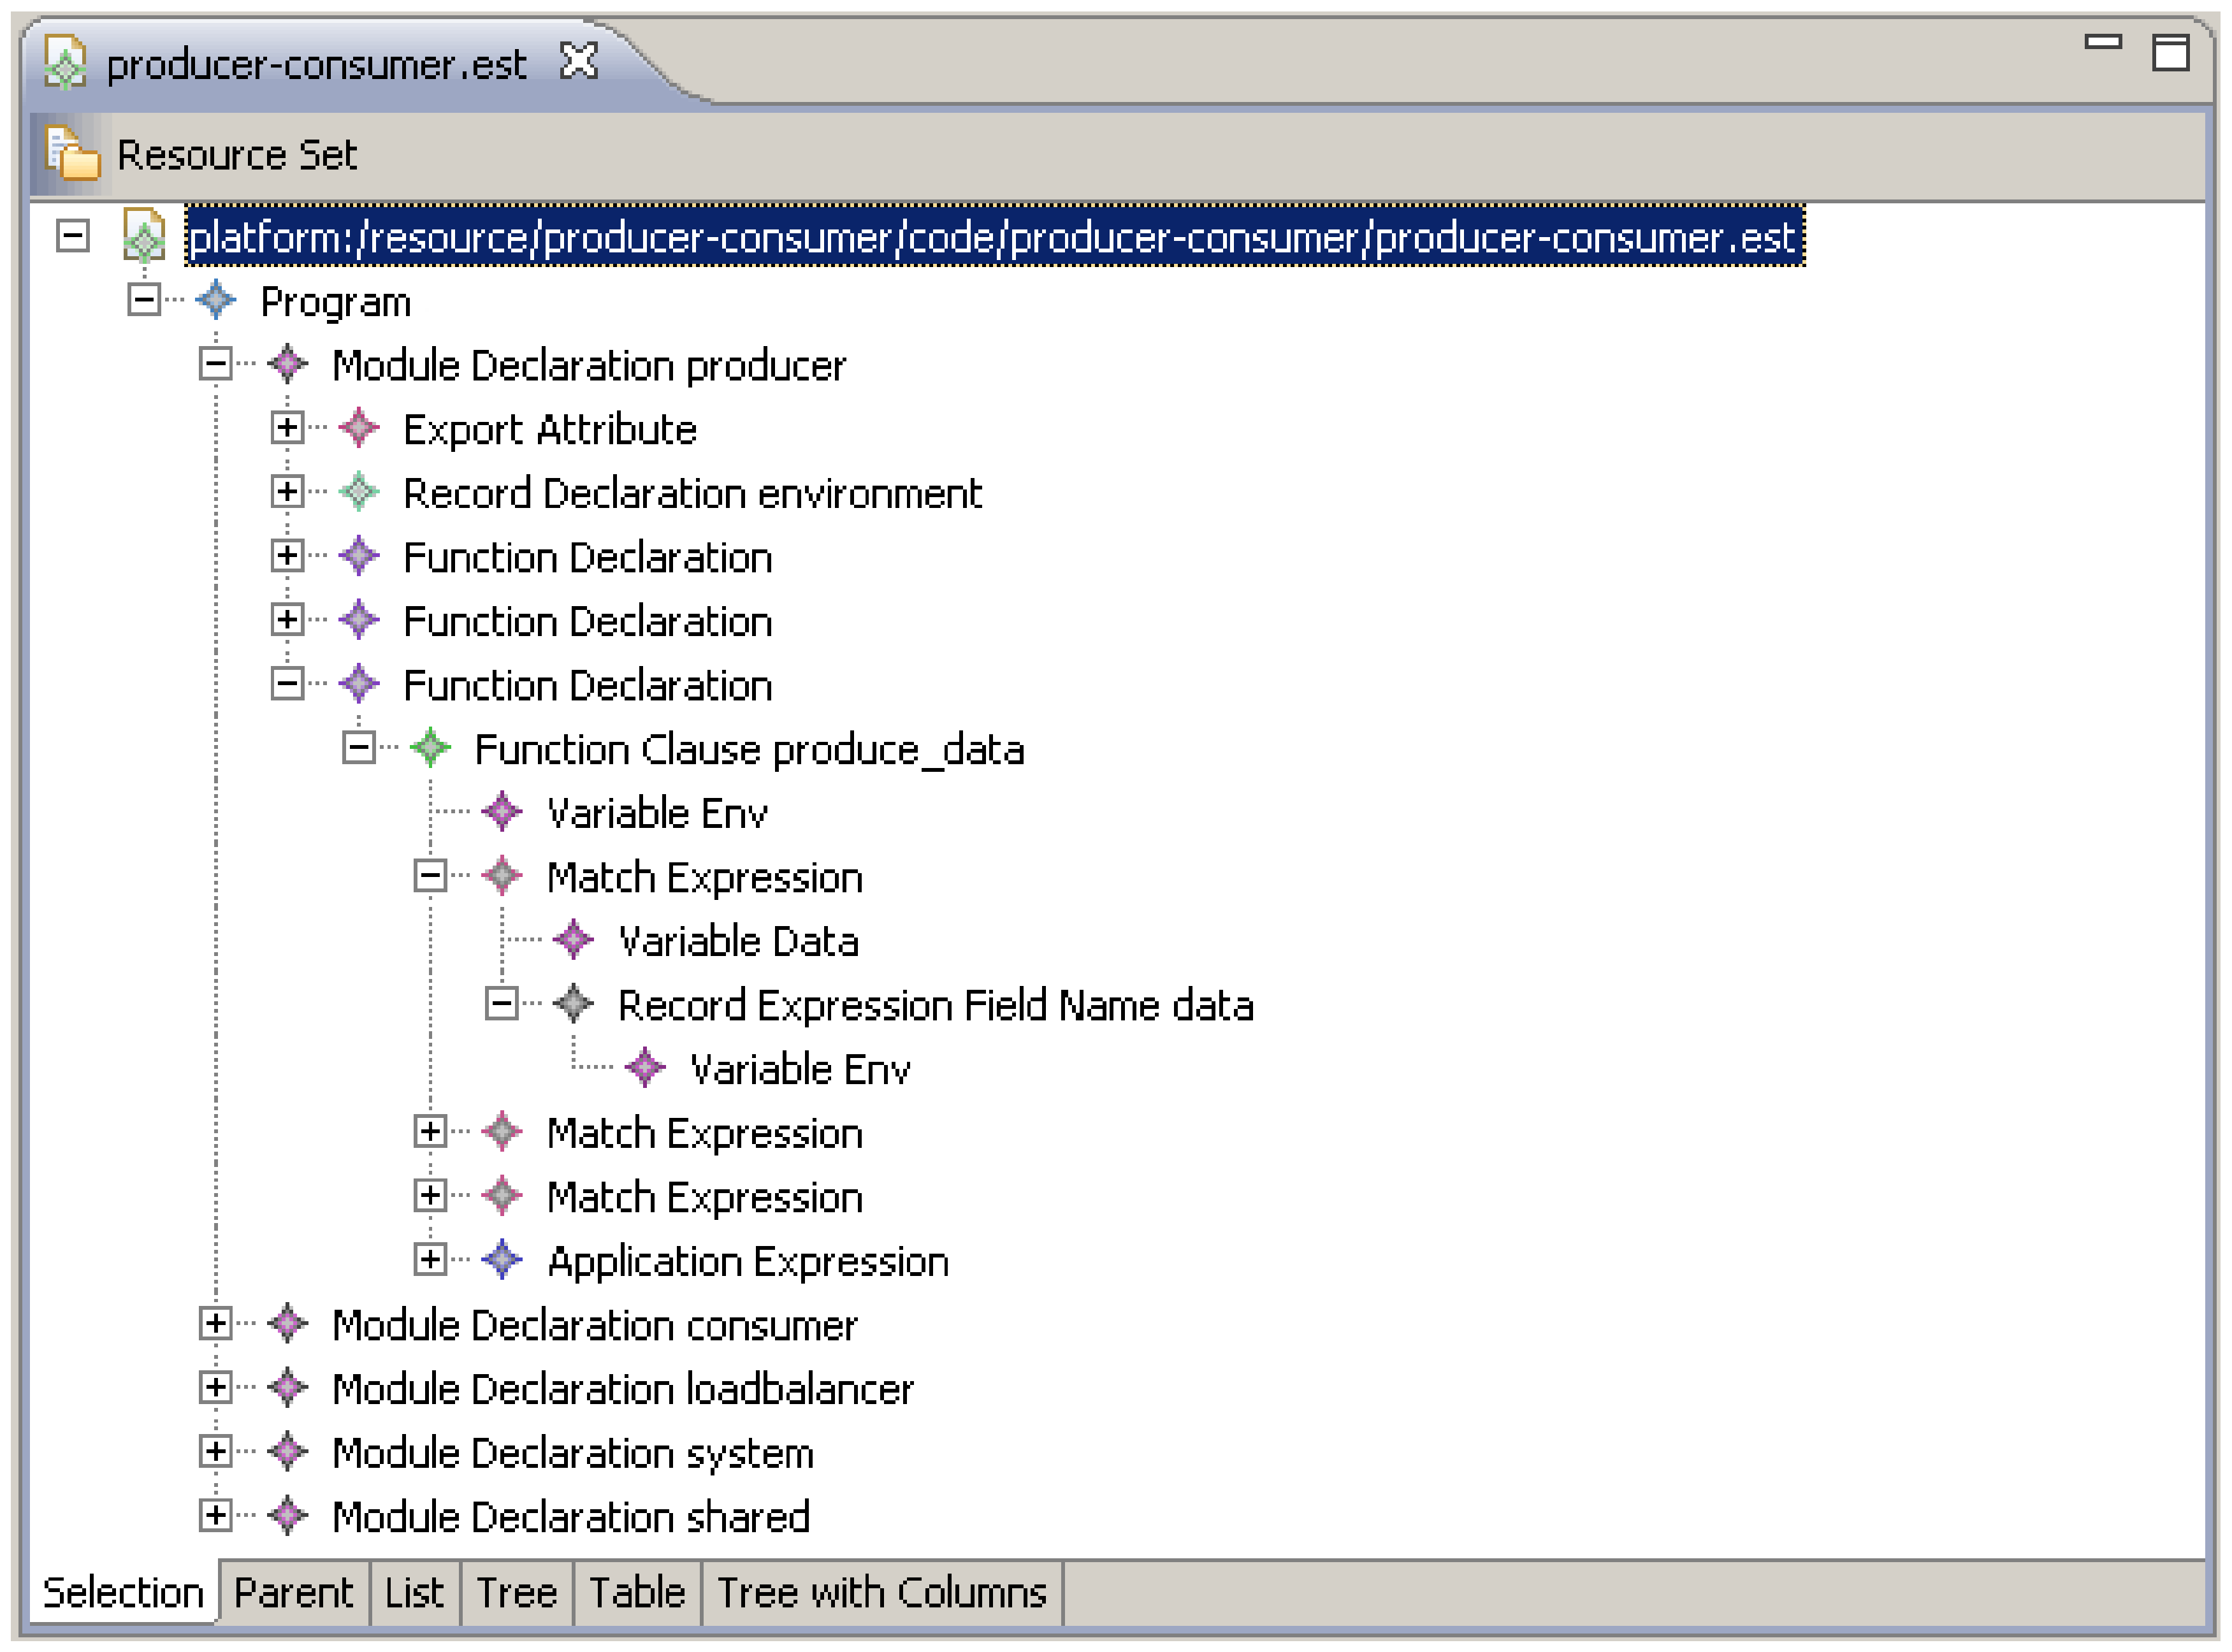
\includegraphics[scale=0.2]{techniques_and_tool/graphics/est.eps}
%\caption{The generated Erlang Syntax Tree (EST)}
%\label{fig:cgest}
%\end{figure}

\subsection{Implementation Details}
We have implemented the tool using the phases described in chapter~\ref{chap:translation}, i.e., CPN $\rightarrow$ decorated CPN $\rightarrow$ CFG $\rightarrow$ AST $\rightarrow$ EST $\rightarrow$ Erlang source code. All phases are completely independent in the implementation in the sense that a given phases takes an EMF model and returns a new EMF model. This showed to be very convenient in the development of the tool. Using the EMF framework it is easy to build, e.g., an example AST and use this model when implementing the AST $\rightarrow$ EST phase. Making the phases independent of each other also has the advantage that is it possible to substitute the Erlang dependent phases with, e.g., Java phases.